\documentclass[sigconf,nonacm]{acmart}
\usepackage{booktabs}
\usepackage{array}
\usepackage{amsmath}
\usepackage{graphicx}
\usepackage{fvextra}
\usepackage{tikz}
\usepackage{pgfplots}
\pgfplotsset{compat=1.18}
\usetikzlibrary{arrows.meta,positioning,calc,fit,backgrounds}
\definecolor{cblu}{RGB}{50,110,190}\definecolor{cgrn}{RGB}{40,150,70}\definecolor{cora}{RGB}{210,110,30}
\definecolor{cred}{RGB}{200,50,50}\definecolor{cgry}{RGB}{100,100,100}\definecolor{cpur}{RGB}{130,50,170}
\setcopyright{none}
\settopmatter{printacmref=false}
\renewcommand\footnotetextcopyrightpermission[1]{}
\title{When Deleted Agent Memories Return: A Controlled Study of Durable Scope Revocation}
\author{Ezekiel Ologunde}
\affiliation{%
  \institution{Independent Researcher}
  \city{Boston}
  \state{MA}
  \country{USA}}
\email{ologunde@bu.edu}
\renewcommand{\shortauthors}{Ologunde}
\begin{document}
\sloppy
\begin{abstract}
External memory deletion is a lifecycle operation: information removed from an active store can return when an earlier snapshot is restored or a previously authorized writer commits. We implement a scope-revocation overlay that combines materialized scope lineage, an independently current deletion authority, commit-time validation, and restore reconciliation. We evaluate six configurations on two persistent reference backends using 140 controlled episodes grounded in public conversational-memory corpora. The experiment comprises 15,120 managed event trials and 560 boundary-control trials, with direct record inspection, persisted-file scans, retrieval probes, and retained-data checks. The full overlay produced zero active record, byte-scan, or retrieval recoveries in 2,520 managed trials. One-time dependency purge was followed by recovery in six of nine event schedules on both backends. The boundary controls demonstrate failure when the authority itself is rolled back or writes bypass interception. Retained replay fixtures remain recoverable. These are deterministic storage-contract results, not measurements of language-model forgetting or deployment-wide erasure. The contribution is an executable, auditable evaluation of revocation durability and its assumptions, together with a portable reference implementation.
\end{abstract}
\keywords{agent memory, data remanence, scope revocation, deletion durability, fault injection}
\maketitle

\section{Introduction}
An instruction to delete a project's memory can involve more than removing the original record. An external-memory pipeline may store a transcript, a compressed summary, a cached response, an index payload, and a checkpoint. Even after these active artifacts are removed, an old snapshot or a queued writer can return the information. The system may acknowledge deletion correctly at one instant while failing to preserve that state through later operations.

This paper investigates a narrow systems question: whether scope-level revocation can remain effective under explicitly controlled lifecycle transitions. It does not attempt to prove that an AI system has forgotten everything about a subject. It separates active-artifact recoverability, retrieval visibility, retained-copy recoverability, and model behavior. Only the first three are measured here. No language model is executed, no model weights are changed, and no semantic embedding inversion is attempted.

Previous work already studies derived-memory residue, counterfactual behavior, mutation-time hooks, and reinjection prevention. Accordingly, neither tombstones nor provenance are claimed as new mechanisms. Our contribution is a reproducible stress protocol that makes restore and write-path assumptions observable, supported by persistent implementations and deliberately failing controls. The result is an initial systems study that can later be extended to production memory frameworks and actual LLM decisions.

We ask: \emph{Under pre-deletion snapshot replay and delayed-write interleavings, does a project-scoped overlay reduce active recoverability compared with source deletion and a one-time dependency purge, while preserving unrelated memory?} Our implementation uses an independently current authority: ordinary memory snapshots do not include or replace its state. The deliberately violated-authority case establishes why that assumption matters.

The study contributes (1) a scoped definition of durable revocation and corresponding state-transition tests; (2) two persistent reference adapters and a configurable overlay; (3) six-arm, two-backend measurements with component ablations; and (4) a result bundle that retains raw trial outcomes, protocol and code hashes, data provenance, and limitations. It does not claim field-wide priority or independent replication of a deployed framework.

\section{Related Work and Positioning}
\subsection{External memory and deletion evaluation}
Chen et al.~\cite{chen2026} examine raw and summary tiers with injected canaries and a forgetting-residue measure. Their versioned HTML describes a 50-instance deletion evaluation and explicitly identifies meaningful facts and additional storage surfaces as extensions. Our study complements that output-oriented measurement with persistent-file inspection and lifecycle transitions. It does not reproduce their model results.

Yang~\cite{yang2026} compares control-plane placement using ForgetEval, including a released adversarial suite and memory adapters. Its limitations discuss substring-scoring artifacts and uneven system capabilities. Mutation-time interception is therefore established prior work. Our contribution concerns the durability contract when old state or old authorization returns, rather than a new semantic deletion planner.

Liu and Li~\cite{liu2026} describe MemScope, paired counterfactual worlds, sham controls, and dependency-aware purge in their publicly indexed abstract. We treat behavioral counterfactual forgetting as overlapping prior work. Because full methods were unavailable during this pass and our experiment executes no LLM, we neither reproduce nor compare numerical behavioral effects.

Wang and Zhang~\cite{memleak2026} distinguish retained correlated information from directly deleted entries in multimodal memory. Such inference is a separate channel: removing linked records does not imply eliminating every fact that can be inferred from legitimate retained context. Our exact synthetic targets diagnose copy reappearance and do not establish semantic non-inference.

\subsection{Lifecycle security and model-side forgetting}
The DSIT-commissioned review~\cite{dsit2026} motivates end-of-lifecycle research, but its January 2026 literature cutoff cannot establish the novelty of later agent-memory work. Chourasia and Shah~\cite{chourasia2023} analyze deletion guarantees in machine learning. Ding et al.~\cite{ding2026} study influence regeneration during continued training in federated agent networks. Our frozen-model storage setting avoids interpreting external-store cleanup as model unlearning.

Shen~\cite{shen2026} uses read-time evidence restoration to diagnose memory eviction. That intervention is distinct from restoring a pre-deletion storage snapshot. The common methodological lesson is to define exactly what restoration changes; an accuracy difference alone does not identify a storage mechanism.

\subsection{Novelty boundary}
The reviewed literature establishes the need to examine derivatives and control-plane operations. Our candidate contribution combines a bounded persistent-store audit, controlled stale-writer and snapshot-replay events, and explicit authority/bypass negative controls. This is a scoped engineering contribution. A claim that this is the first such system would require broader searches and complete comparison with overlapping frameworks, which are not established by this experiment.

\section{System Model and Deletion Contract}
\subsection{Artifacts, scopes, and the current authority}
Let an artifact be $a=(i,\ell,c,P,G)$, where $i$ is an opaque identifier, $\ell$ its storage layer, $c$ its content, $P$ its parent identifiers, and $G$ a mapping of scope identifiers to the generations under which it was created. A record may depend on more than one scope. The prototype stores materialized scope membership on every derivative; its purge selects that membership directly. It does not infer or traverse an unknown dependency graph.

For each scope $s$, the authority stores $D(s)=(e_s,r_s)$, with generation $e_s$ and a revocation flag $r_s$. A never-revoked scope defaults to $(0,\mathrm{false})$. Artifact admission requires
\begin{equation}
 \operatorname{admit}(a,D)=\bigwedge_{s\in\operatorname{dom}(G_a)}
 [\neg r_s\ \land\ G_a(s)=e_s].
\label{eq:admit}
\end{equation}
Deletion advances the scope generation and marks it revoked. The first prototype has no reauthorization API: a legitimate new disclosure would require an explicitly specified policy and new generation assignment. Blocking an old scope indefinitely is not presented as a complete product policy.

The authority is stored separately from the memory snapshot. This is an assumption of the protocol, not an intrinsic property of JSON files. Atomic replacement protects file-update structure under tested operation; the prototype does not implement a distributed transaction, power-loss synchronization guarantee, or hardware rollback-resistant counter.

\subsection{Operations}
The full overlay performs four actions. First, it records revocation. Second, it removes active artifacts carrying the target scope, including the source and materialized derivatives. Third, every managed writer validates its artifact generation when committing. Fourth, restore filters snapshot contents against the current authority before publishing them into the active store. The materialized index is rebuilt from the resulting records. Figure~\ref{fig:arch} summarizes these actions, the authority, and the events they guard against.

\begin{figure*}[t]
\centering
\resizebox{\textwidth}{!}{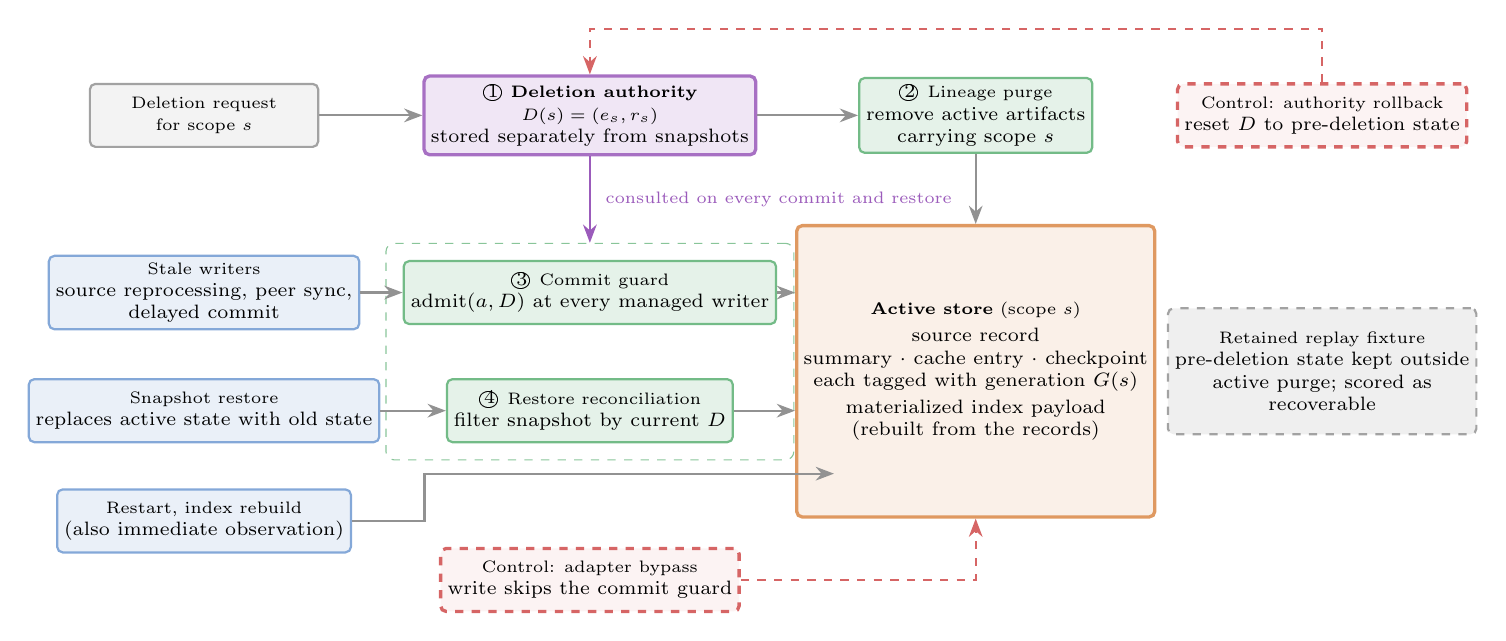
\begin{tikzpicture}[font=\fontsize{6.5pt}{8pt}\selectfont, >=Stealth,
  box/.style={rectangle, rounded corners=2pt, draw=cgry!60, thick, fill=cgry!8, minimum width=2.9cm, minimum height=0.8cm, text centered, align=center, inner sep=2.5pt},
  ev/.style={box, draw=cblu!60, fill=cblu!10},
  guard/.style={box, draw=cgrn!65, fill=cgrn!12},
  auth/.style={box, draw=cpur!70, very thick, fill=cpur!12, minimum width=3.6cm, minimum height=1.0cm},
  store/.style={box, draw=cora!70, very thick, fill=cora!10, minimum width=3.6cm, minimum height=3.7cm},
  act/.style={box, draw=cgrn!65, fill=cgrn!12},
  ctl/.style={box, draw=cred!75, dashed, very thick, fill=cred!6},
  fix/.style={box, draw=cgry!60, dashed, thick, fill=cgry!10, minimum width=3.0cm, minimum height=1.6cm},
  arr/.style={-{Stealth}, thick, cgry!70},
  carr/.style={-{Stealth}, thick, cred!75, dashed}]
\node[box] (req) at (0,3.6) {Deletion request\\ for scope $s$};
\node[auth] (auth) at (4.9,3.6) {\textcircled{\scriptsize 1} \textbf{Deletion authority}\\ $D(s)=(e_s,r_s)$\\ \scriptsize stored separately from snapshots};
\node[act] (purge) at (9.8,3.6) {\textcircled{\scriptsize 2} Lineage purge\\ \scriptsize remove active artifacts\\ \scriptsize carrying scope $s$};
\node[store] (store) at (9.8,0.35) {\textbf{Active store} (scope $s$)\\[2pt] \scriptsize source record\\ \scriptsize summary $\cdot$ cache entry $\cdot$ checkpoint\\ \scriptsize each tagged with generation $G(s)$\\[2pt] \scriptsize materialized index payload\\ \scriptsize (rebuilt from the records)};
\node[guard] (g1) at (4.9,1.35) {\textcircled{\scriptsize 3} Commit guard\\ \scriptsize admit$(a,D)$ at every managed writer};
\node[guard] (g2) at (4.9,-0.15) {\textcircled{\scriptsize 4} Restore reconciliation\\ \scriptsize filter snapshot by current $D$};
\begin{scope}[on background layer]
\node[draw=cgrn!55, dashed, rounded corners=3pt, fit=(g1)(g2), inner sep=6pt] (enf) {};
\end{scope}
\node[ev] (e1) at (0,1.35) {Stale writers\\ \scriptsize source reprocessing, peer sync,\\ \scriptsize delayed commit};
\node[ev] (e2) at (0,-0.15) {Snapshot restore\\ \scriptsize replaces active state with old state};
\node[ev] (e3) at (0,-1.55) {Restart, index rebuild\\ \scriptsize (also immediate observation)};
\node[ctl] (c1) at (4.9,-2.3) {Control: adapter bypass\\ \scriptsize write skips the commit guard};
\node[ctl] (c2) at (14.2,3.6) {Control: authority rollback\\ \scriptsize reset $D$ to pre-deletion state};
\node[fix] (fx) at (14.2,0.35) {Retained replay fixture\\ \scriptsize pre-deletion state kept outside\\ \scriptsize active purge; scored as\\ \scriptsize recoverable};
\draw[arr] (req) -- (auth);
\draw[arr] (auth) -- (purge);
\draw[arr] (purge) -- (store);
\draw[arr, cpur!80] (auth.south) -- node[right=2pt, font=\fontsize{5.6pt}{7pt}\selectfont, text=cpur!80] {consulted on every commit and restore} (enf.north);
\draw[arr] (e1) -- (g1);
\draw[arr] (e2) -- (g2);
\draw[arr] (g1.east) -- (store.west |- g1.east);
\draw[arr] (g2.east) -- (store.west |- g2.east);
\draw[arr] (e3.east) -- (2.8,-1.55) -- (2.8,-0.95) -- (8.0,-0.95);
\draw[carr] (c1.east) -- (9.8,-2.3) -- (store.south);
\draw[carr] (c2.north) -- (14.2,4.7) -- (4.9,4.7) -- (auth.north);
\end{tikzpicture}}
\caption{Overlay architecture and the events it must survive. A deletion request advances the scope generation and revokes it in an authority kept separate from memory snapshots (step 1), then purges active artifacts carrying the scope (step 2). Two guards enforce the authority afterwards: a commit guard on every managed writer (step 3) and a reconciliation filter on restored snapshots (step 4). Blue boxes are the lifecycle events exercised in the experiment; red dashed boxes are the two boundary controls that violate the protocol's assumptions (authority rolled back; write path bypassing the guard). The retained replay fixture lies outside the active store and is scored as recoverable. This is a structural diagram of the design described in Section~3; it contains no measured values.}
\Description{Block diagram of the overlay. A deletion request updates the deletion authority, which is stored separately from memory snapshots, and triggers a lineage purge of the active store. A commit guard on managed writers and a restore reconciliation filter, both consulting the authority, sit between lifecycle events (stale writers, snapshot restore) and the active store. Restart and index rebuild act on the store directly. Two red dashed boxes mark boundary controls: authority rollback targets the authority, and adapter bypass writes to the store without passing the commit guard. A retained replay fixture sits outside the active store.}
\label{fig:arch}
\end{figure*}


The test coordinator serializes authority checks and writes. A check followed by an unprotected concurrent write in a production system can still race with revocation. Production integration would require a transaction, lock, or compare-and-swap spanning authorization and publication. Our controlled delayed-write schedule verifies the decision at the commit boundary; it is not a proof of concurrent linearizability.

\subsection{Success and boundaries}
Active revocation succeeds for a tested event if the synthetic target is absent from the active record content and its materialized index payload. Persisted-file absence is measured separately by scanning all currently reachable files in the active adapter directory. Those scans include SQLite database, WAL/shared-memory files when present, and the index sidecar, or JSON record/index files. They do not inspect released filesystem blocks, operating-system page caches, SSD firmware, remote telemetry, or all physical media.

A retained snapshot is a different object. Our fault-replay fixture deliberately retains the pre-deletion state so that restoration is testable. It remains outside active purge and is explicitly scored as recoverable. An effective restore gate can prevent that old content from becoming active while its retained bytes still exist. Therefore the study establishes scoped revocation, not whole-system erasure.

\section{Implementation}
\subsection{Persistent adapters}
The SQLite adapter stores JSON artifact payloads in a relational table and maintains an FTS5 table. It uses WAL mode, \texttt{synchronous=FULL}, and \texttt{secure\_delete=ON}. Purge performs checkpoint/truncation, \texttt{VACUUM}, and a second checkpoint. SQLite's documentation distinguishes active database content from WAL behavior and notes limits of secure deletion, including virtual-table shadow structures~\cite{sqlitepragma,sqlitewal}. We scan the actual files rather than treating a pragma as proof of erasure.

The filesystem adapter stores records in a JSON file using write-to-pending followed by atomic replacement. Both adapters persist a materialized index containing record IDs, content payloads, scope labels, and numerical vectors. The index is intentionally transparent so that a stale payload can be independently detected. It is not a Qdrant, Chroma, Mem0, or Letta implementation, and results must not be attributed to those products.

\subsection{Retrieval and derivative construction}
Retrieval uses a 128-dimensional hashed lexical vector. Tokens are lowercase ASCII alphanumeric/underscore matches; SHA-256 selects a dimension and sign, term counts accumulate, and vectors are normalized for cosine ranking. Tie-breaking uses the opaque record ID. This deterministic projection is not a learned embedding, does not model semantic paraphrase retrieval, and provides no embedding-inversion result.

Each injected project source has three deterministic copies: a summary, cache entry, and checkpoint record. They preserve the target token and preference statement. These fixtures deliberately guarantee a deletion dependency; they are not outputs of an LLM summarizer. The experiment therefore tests whether known copied content is removed and prevented from returning. It cannot estimate how often an actual summarizer creates such copies.

\subsection{Validation and reproducibility}
Eighteen implementation tests cover immediate purge, stale commit rejection, restore reconciliation, authority restart, repeated deletion, scope isolation, index consistency, and the two failing boundary controls. One test removes a derivative whose text does not contain the source token, verifying that scope selection does not rely solely on literal matching. Tests execute both adapters where appropriate.

The main run records protocol/code/data hashes, platform and SQLite versions, each trial's outcome, marker-containing active filenames, acquisition status, utility checks, and operation timings. Semantic agreement across adapters is audited separately from timing and physical-layout differences. Four processes execute disjoint episode shards in independent directories. Timing measurements therefore reflect a shared-host batch run, not isolated throughput or a production performance benchmark.

\section{Experimental Design}
\subsection{Data and sampling}
LongMemEval~\cite{longmemeval} supplies 500 questions in the downloaded cleaned oracle release. We choose 20 questions from each of its six question-type fields using a fixed SHA-256 ordering over question identifiers, giving 120 episodes. All available oracle sessions for each chosen question become background raw records. Abstention items are not excluded from deletion tests; items without evidence do not contribute to gold-evidence recall.

LoCoMo~\cite{locomo} supplies ten conversation histories in the downloaded release. We choose two questions with nonempty answers and evidence per conversation using a fixed hash ordering, adding 20 episodes. All conversation sessions become background records for the selected question. These two questions per conversation are related, so their repetitions are not treated as 20 independent deployment populations.

Original session identifiers can carry answer text. We replace them with opaque record identifiers before indexing and keep their evidence mapping in evaluator-only metadata. The injected token is a deterministic 24-hex-character suffix of a hash over a study-specific prefix and episode ID. It is unique in this finite experiment but public and reproducible; no actual credential is inserted.

Each episode adds Project X with the target token and a route preference, plus an unrelated Project Y meeting-day control. Project X's target and all its prepared copies start at generation zero. The question's original background sessions provide corpus diversity and a retained-retrieval check; they do not turn the synthetic fault schedule into a representative real-world distribution.

\subsection{Comparison arms}
\begin{table}[t]
\caption{Six configurations. All use the same artifact state, compaction policy, and retrieval procedure. Source deletion is a reference adapter operation, not a claim about a vendor's scope-deletion API.}
\label{tab:arms}
\begin{tabular}{>{\raggedright\arraybackslash}p{0.27\linewidth}>{\raggedright\arraybackslash}p{0.64\linewidth}}
\toprule
Configuration & Operation \\
\midrule
Source deletion & Remove original record only; derivatives remain. \\
Dependency purge & Remove all active records with target scope once. \\
Full overlay & Purge, current authority, commit guard, restore reconciliation. \\
Without commit guard & Full overlay except stale writers are admitted. \\
Without restore guard & Full overlay except old snapshots are published unfiltered. \\
Without lineage purge & Revoke and guard future operations, but remove only the source immediately. \\
\bottomrule
\end{tabular}
\end{table}
The source-only arm tests an intentionally incomplete operation and serves as a positive residue control. The more informative comparator is dependency purge, which removes all known active copies and shares the same storage cleanup. No comparison is made to the performance of a proprietary native deletion service.

\subsection{Lifecycle events and negative controls}
Each configuration is tested under nine schedules: immediate observation; adapter restart; index rebuild; original-source reprocessing; pre-deletion snapshot restoration; delayed commit of a pre-deletion artifact; peer-copy synchronization with a newly minted ID; restore followed by stale commit; and stale commit followed by restart. Snapshot restoration replaces active state with the recorded old state unless the restore guard filters it. Reprocessing and sync submit an old-generation artifact through the managed commit path.

Two additional schedules apply only to the full overlay. Authority rollback replaces the deletion authority with its pre-deletion empty state and restores old memory. Adapter bypass writes a queued artifact while explicitly skipping the guard. These are expected failure controls: they challenge the assumptions required for revocation and must not be hidden in a favorable managed-event average.

The grid is $140\times2\times6\times9=15{,}120$ managed trials, plus $140\times2\times2=560$ boundary trials. The 15,680 trials are not 15,680 independent agents. Each trial starts by reinitializing the same episode state; read-only probes do not mutate it. Each processed episode verifies pre-deletion acquisition and retrieval so that an empty or never-learned target cannot pass deletion vacuously.

\subsection{Measurements and hypotheses}
For episode $i$, configuration $m$, backend $b$, and event $e$, define active record recovery
\begin{equation}
 R_{imbe}=\mathbf{1}\{c_i\text{ occurs in an active artifact or index payload}\}.
\end{equation}
The worst-event endpoint is $W_{imb}=\max_e R_{imbe}$ over the nine managed schedules. We also record target recovery in the top-three retrieval payloads, exact marker presence in persisted active files, literal project-preference residue, unrelated-control preservation, and unmodified background records.

Retained utility is measured as unchanged top-three ranking of raw records relative to the same background plus Project Y without Project X, and gold-session recall where an evidence mapping exists. This is a retrieval-preservation proxy, not generated-answer accuracy, personalization utility, or behavioral equivalence.

H1 predicts that a one-time purge can pass immediately and fail after an event. H2 predicts lower worst-event recovery with the full overlay. H3 predicts event-specific failure when its corresponding guard is removed. H4 predicts preservation of unrelated artifacts and matched retrieval. The protocol was saved locally before the main measurement; it was not registered with an external preregistration service. Runtime smoke tests preceded the full run and were used to address Windows file-sharing retries and caching, not to select favorable paper outcomes.

\subsection{Analysis scope}
We report exact finite-grid counts and event-level patterns. A paired episode bootstrap with 10,000 resamples characterizes the observed worst-event contrast. Identical deterministic episode contrasts can produce a degenerate interval; that interval describes this test set and is not a bound on unseen deployment risk. Repeating the same target across events or backends does not create independent statistical evidence. A zero-event rate cannot establish universal forgetting.

\section{Results}
All 15,680 trials acquired the target before deletion. Trial keys were unique, recorded code and protocol hashes matched, and semantic outcomes agreed across backends. The full overlay yielded 0/2,520 active-record recoveries, 0/2,520 persisted-byte recoveries, and 0/2,520 top-three retrieval recoveries. These counts concern the enumerated managed artifacts, not every storage surface of an AI service. Table~\ref{tab:events} reports the deterministic event pattern.

\begin{table}[t]
\caption{Active record/index recovery by event, expressed as percentages over 140 episodes per backend. Both backends produce the same values. I: immediate; RS: restart; IX: rebuild; SP: source reprocessing; SR: snapshot restore; DC: delayed commit; PS: peer sync; SC: restore then commit; CR: commit then restart.}
\label{tab:events}
\centering\small\setlength{\tabcolsep}{2.4pt}
\begin{tabular}{lrrrrrrrrr}
\toprule
Configuration & I & RS & IX & SP & SR & DC & PS & SC & CR \\
\midrule
Source-only deletion & 100 & 100 & 100 & 100 & 100 & 100 & 100 & 100 & 100 \\
Dependency purge & 0 & 0 & 0 & 100 & 100 & 100 & 100 & 100 & 100 \\
Full overlay & 0 & 0 & 0 & 0 & 0 & 0 & 0 & 0 & 0 \\
No commit guard & 0 & 0 & 0 & 100 & 0 & 100 & 100 & 100 & 100 \\
No restore guard & 0 & 0 & 0 & 0 & 100 & 0 & 0 & 100 & 0 \\
No lineage purge & 100 & 100 & 100 & 100 & 0 & 100 & 100 & 0 & 100 \\
\bottomrule
\end{tabular}
\end{table}

Figure~\ref{fig:heat} shows the same values as a heat map and adds the two boundary controls.

\begin{figure}[t]
\centering
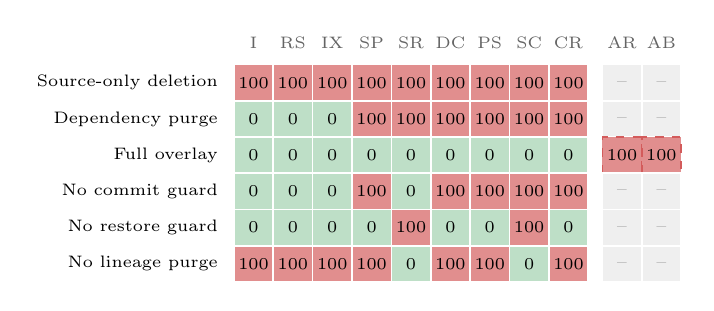
\begin{tikzpicture}[font=\fontsize{6.2pt}{7.4pt}\selectfont]
\node[text=cgry] at (2.800,0.28) {I};
\node[text=cgry] at (3.300,0.28) {RS};
\node[text=cgry] at (3.800,0.28) {IX};
\node[text=cgry] at (4.300,0.28) {SP};
\node[text=cgry] at (4.800,0.28) {SR};
\node[text=cgry] at (5.300,0.28) {DC};
\node[text=cgry] at (5.800,0.28) {PS};
\node[text=cgry] at (6.300,0.28) {SC};
\node[text=cgry] at (6.800,0.28) {CR};
\node[text=cgry] at (7.480,0.28) {AR};
\node[text=cgry] at (7.980,0.28) {AB};
\node[anchor=east] at (2.47,-0.230) {Source-only deletion};
\fill[cred!55, draw=white, line width=0.6pt] (2.550,-0.460) rectangle (3.050,0.000);
\node at (2.800,-0.230) {100};
\fill[cred!55, draw=white, line width=0.6pt] (3.050,-0.460) rectangle (3.550,0.000);
\node at (3.300,-0.230) {100};
\fill[cred!55, draw=white, line width=0.6pt] (3.550,-0.460) rectangle (4.050,0.000);
\node at (3.800,-0.230) {100};
\fill[cred!55, draw=white, line width=0.6pt] (4.050,-0.460) rectangle (4.550,0.000);
\node at (4.300,-0.230) {100};
\fill[cred!55, draw=white, line width=0.6pt] (4.550,-0.460) rectangle (5.050,0.000);
\node at (4.800,-0.230) {100};
\fill[cred!55, draw=white, line width=0.6pt] (5.050,-0.460) rectangle (5.550,0.000);
\node at (5.300,-0.230) {100};
\fill[cred!55, draw=white, line width=0.6pt] (5.550,-0.460) rectangle (6.050,0.000);
\node at (5.800,-0.230) {100};
\fill[cred!55, draw=white, line width=0.6pt] (6.050,-0.460) rectangle (6.550,0.000);
\node at (6.300,-0.230) {100};
\fill[cred!55, draw=white, line width=0.6pt] (6.550,-0.460) rectangle (7.050,0.000);
\node at (6.800,-0.230) {100};
\fill[cgry!10, draw=white, line width=0.6pt] (7.230,-0.460) rectangle (7.730,0.000);
\node[text=cgry!60] at (7.480,-0.230) {--};
\fill[cgry!10, draw=white, line width=0.6pt] (7.730,-0.460) rectangle (8.230,0.000);
\node[text=cgry!60] at (7.980,-0.230) {--};
\node[anchor=east] at (2.47,-0.690) {Dependency purge};
\fill[cgrn!30, draw=white, line width=0.6pt] (2.550,-0.920) rectangle (3.050,-0.460);
\node at (2.800,-0.690) {0};
\fill[cgrn!30, draw=white, line width=0.6pt] (3.050,-0.920) rectangle (3.550,-0.460);
\node at (3.300,-0.690) {0};
\fill[cgrn!30, draw=white, line width=0.6pt] (3.550,-0.920) rectangle (4.050,-0.460);
\node at (3.800,-0.690) {0};
\fill[cred!55, draw=white, line width=0.6pt] (4.050,-0.920) rectangle (4.550,-0.460);
\node at (4.300,-0.690) {100};
\fill[cred!55, draw=white, line width=0.6pt] (4.550,-0.920) rectangle (5.050,-0.460);
\node at (4.800,-0.690) {100};
\fill[cred!55, draw=white, line width=0.6pt] (5.050,-0.920) rectangle (5.550,-0.460);
\node at (5.300,-0.690) {100};
\fill[cred!55, draw=white, line width=0.6pt] (5.550,-0.920) rectangle (6.050,-0.460);
\node at (5.800,-0.690) {100};
\fill[cred!55, draw=white, line width=0.6pt] (6.050,-0.920) rectangle (6.550,-0.460);
\node at (6.300,-0.690) {100};
\fill[cred!55, draw=white, line width=0.6pt] (6.550,-0.920) rectangle (7.050,-0.460);
\node at (6.800,-0.690) {100};
\fill[cgry!10, draw=white, line width=0.6pt] (7.230,-0.920) rectangle (7.730,-0.460);
\node[text=cgry!60] at (7.480,-0.690) {--};
\fill[cgry!10, draw=white, line width=0.6pt] (7.730,-0.920) rectangle (8.230,-0.460);
\node[text=cgry!60] at (7.980,-0.690) {--};
\node[anchor=east] at (2.47,-1.150) {Full overlay};
\fill[cgrn!30, draw=white, line width=0.6pt] (2.550,-1.380) rectangle (3.050,-0.920);
\node at (2.800,-1.150) {0};
\fill[cgrn!30, draw=white, line width=0.6pt] (3.050,-1.380) rectangle (3.550,-0.920);
\node at (3.300,-1.150) {0};
\fill[cgrn!30, draw=white, line width=0.6pt] (3.550,-1.380) rectangle (4.050,-0.920);
\node at (3.800,-1.150) {0};
\fill[cgrn!30, draw=white, line width=0.6pt] (4.050,-1.380) rectangle (4.550,-0.920);
\node at (4.300,-1.150) {0};
\fill[cgrn!30, draw=white, line width=0.6pt] (4.550,-1.380) rectangle (5.050,-0.920);
\node at (4.800,-1.150) {0};
\fill[cgrn!30, draw=white, line width=0.6pt] (5.050,-1.380) rectangle (5.550,-0.920);
\node at (5.300,-1.150) {0};
\fill[cgrn!30, draw=white, line width=0.6pt] (5.550,-1.380) rectangle (6.050,-0.920);
\node at (5.800,-1.150) {0};
\fill[cgrn!30, draw=white, line width=0.6pt] (6.050,-1.380) rectangle (6.550,-0.920);
\node at (6.300,-1.150) {0};
\fill[cgrn!30, draw=white, line width=0.6pt] (6.550,-1.380) rectangle (7.050,-0.920);
\node at (6.800,-1.150) {0};
\fill[cred!55, draw=cred!80, dashed, line width=0.6pt] (7.230,-1.380) rectangle (7.730,-0.920);
\node at (7.480,-1.150) {100};
\fill[cred!55, draw=cred!80, dashed, line width=0.6pt] (7.730,-1.380) rectangle (8.230,-0.920);
\node at (7.980,-1.150) {100};
\node[anchor=east] at (2.47,-1.610) {No commit guard};
\fill[cgrn!30, draw=white, line width=0.6pt] (2.550,-1.840) rectangle (3.050,-1.380);
\node at (2.800,-1.610) {0};
\fill[cgrn!30, draw=white, line width=0.6pt] (3.050,-1.840) rectangle (3.550,-1.380);
\node at (3.300,-1.610) {0};
\fill[cgrn!30, draw=white, line width=0.6pt] (3.550,-1.840) rectangle (4.050,-1.380);
\node at (3.800,-1.610) {0};
\fill[cred!55, draw=white, line width=0.6pt] (4.050,-1.840) rectangle (4.550,-1.380);
\node at (4.300,-1.610) {100};
\fill[cgrn!30, draw=white, line width=0.6pt] (4.550,-1.840) rectangle (5.050,-1.380);
\node at (4.800,-1.610) {0};
\fill[cred!55, draw=white, line width=0.6pt] (5.050,-1.840) rectangle (5.550,-1.380);
\node at (5.300,-1.610) {100};
\fill[cred!55, draw=white, line width=0.6pt] (5.550,-1.840) rectangle (6.050,-1.380);
\node at (5.800,-1.610) {100};
\fill[cred!55, draw=white, line width=0.6pt] (6.050,-1.840) rectangle (6.550,-1.380);
\node at (6.300,-1.610) {100};
\fill[cred!55, draw=white, line width=0.6pt] (6.550,-1.840) rectangle (7.050,-1.380);
\node at (6.800,-1.610) {100};
\fill[cgry!10, draw=white, line width=0.6pt] (7.230,-1.840) rectangle (7.730,-1.380);
\node[text=cgry!60] at (7.480,-1.610) {--};
\fill[cgry!10, draw=white, line width=0.6pt] (7.730,-1.840) rectangle (8.230,-1.380);
\node[text=cgry!60] at (7.980,-1.610) {--};
\node[anchor=east] at (2.47,-2.070) {No restore guard};
\fill[cgrn!30, draw=white, line width=0.6pt] (2.550,-2.300) rectangle (3.050,-1.840);
\node at (2.800,-2.070) {0};
\fill[cgrn!30, draw=white, line width=0.6pt] (3.050,-2.300) rectangle (3.550,-1.840);
\node at (3.300,-2.070) {0};
\fill[cgrn!30, draw=white, line width=0.6pt] (3.550,-2.300) rectangle (4.050,-1.840);
\node at (3.800,-2.070) {0};
\fill[cgrn!30, draw=white, line width=0.6pt] (4.050,-2.300) rectangle (4.550,-1.840);
\node at (4.300,-2.070) {0};
\fill[cred!55, draw=white, line width=0.6pt] (4.550,-2.300) rectangle (5.050,-1.840);
\node at (4.800,-2.070) {100};
\fill[cgrn!30, draw=white, line width=0.6pt] (5.050,-2.300) rectangle (5.550,-1.840);
\node at (5.300,-2.070) {0};
\fill[cgrn!30, draw=white, line width=0.6pt] (5.550,-2.300) rectangle (6.050,-1.840);
\node at (5.800,-2.070) {0};
\fill[cred!55, draw=white, line width=0.6pt] (6.050,-2.300) rectangle (6.550,-1.840);
\node at (6.300,-2.070) {100};
\fill[cgrn!30, draw=white, line width=0.6pt] (6.550,-2.300) rectangle (7.050,-1.840);
\node at (6.800,-2.070) {0};
\fill[cgry!10, draw=white, line width=0.6pt] (7.230,-2.300) rectangle (7.730,-1.840);
\node[text=cgry!60] at (7.480,-2.070) {--};
\fill[cgry!10, draw=white, line width=0.6pt] (7.730,-2.300) rectangle (8.230,-1.840);
\node[text=cgry!60] at (7.980,-2.070) {--};
\node[anchor=east] at (2.47,-2.530) {No lineage purge};
\fill[cred!55, draw=white, line width=0.6pt] (2.550,-2.760) rectangle (3.050,-2.300);
\node at (2.800,-2.530) {100};
\fill[cred!55, draw=white, line width=0.6pt] (3.050,-2.760) rectangle (3.550,-2.300);
\node at (3.300,-2.530) {100};
\fill[cred!55, draw=white, line width=0.6pt] (3.550,-2.760) rectangle (4.050,-2.300);
\node at (3.800,-2.530) {100};
\fill[cred!55, draw=white, line width=0.6pt] (4.050,-2.760) rectangle (4.550,-2.300);
\node at (4.300,-2.530) {100};
\fill[cgrn!30, draw=white, line width=0.6pt] (4.550,-2.760) rectangle (5.050,-2.300);
\node at (4.800,-2.530) {0};
\fill[cred!55, draw=white, line width=0.6pt] (5.050,-2.760) rectangle (5.550,-2.300);
\node at (5.300,-2.530) {100};
\fill[cred!55, draw=white, line width=0.6pt] (5.550,-2.760) rectangle (6.050,-2.300);
\node at (5.800,-2.530) {100};
\fill[cgrn!30, draw=white, line width=0.6pt] (6.050,-2.760) rectangle (6.550,-2.300);
\node at (6.300,-2.530) {0};
\fill[cred!55, draw=white, line width=0.6pt] (6.550,-2.760) rectangle (7.050,-2.300);
\node at (6.800,-2.530) {100};
\fill[cgry!10, draw=white, line width=0.6pt] (7.230,-2.760) rectangle (7.730,-2.300);
\node[text=cgry!60] at (7.480,-2.530) {--};
\fill[cgry!10, draw=white, line width=0.6pt] (7.730,-2.760) rectangle (8.230,-2.300);
\node[text=cgry!60] at (7.980,-2.530) {--};
\end{tikzpicture}
\caption{Active record/index recovery by configuration and schedule, generated directly from \texttt{cell-results.csv} (140 episodes per cell; SQLite WAL and JSON-file backends agree in every cell). Red cells: the target was recovered in every episode; green cells: in none. Columns I--CR are the nine managed schedules of Table~\ref{tab:events}; AR (authority rollback) and AB (adapter bypass) are the boundary controls, run only for the full overlay (dashed outline; ``--'' means not run).}
\Description{Heat map with six configuration rows and eleven columns: nine managed schedules and two boundary controls. Source-only deletion is red in 9 of 9 managed schedules (I, RS, IX, SP, SR, DC, PS, SC, CR). Dependency purge is red in 6 of 9 managed schedules (SP, SR, DC, PS, SC, CR). Full overlay is red in 0 of 9 managed schedules (none). No commit guard is red in 5 of 9 managed schedules (SP, DC, PS, SC, CR). No restore guard is red in 2 of 9 managed schedules (SR, SC). No lineage purge is red in 7 of 9 managed schedules (I, RS, IX, SP, DC, PS, CR). The full overlay is red under both boundary controls (authority rollback 100 percent, adapter bypass 100 percent).}
\label{fig:heat}
\end{figure}

\subsection{Immediate success and later reappearance}
Dependency purge passed immediate, restart, and index-rebuild checks but failed all 140 episodes under each of the other six event schedules, on each backend: 840/1,260 managed trials per backend (66.7\%). All 140 episodes had at least one post-deletion recovery. Source-only deletion failed all nine schedules because surviving derivatives retained the target. A clean active-state observation is thus compatible with later failure. The source-reprocessing and peer-copy schedules create a new ID, showing why record-specific removal is insufficient when a writer can recreate old content under a different identity. The tested scope epoch supplies the relevant authorization boundary.

\subsection{Guard ablations}
Removing the commit guard caused recovery in five schedules (700/1,260 trials per backend); removing restore reconciliation caused recovery in two (280/1,260); removing lineage purge caused recovery in seven (980/1,260). The paired episode-level worst-event contrast between full overlay and dependency purge was $-1.00$ on each backend; its descriptive percentile bootstrap interval was $[-1.00,-1.00]$. This degenerate interval reflects identical controlled episode outcomes. These event-specific effects support the implementation mechanism under controlled interleavings. They do not imply that the same rates occur in ordinary deployments. The events deliberately exercise the behavior each guard is designed to prevent.

Figure~\ref{fig:bars} plots pooled recovery per configuration, with the two boundary controls alongside.

\begin{figure}[t]
\centering
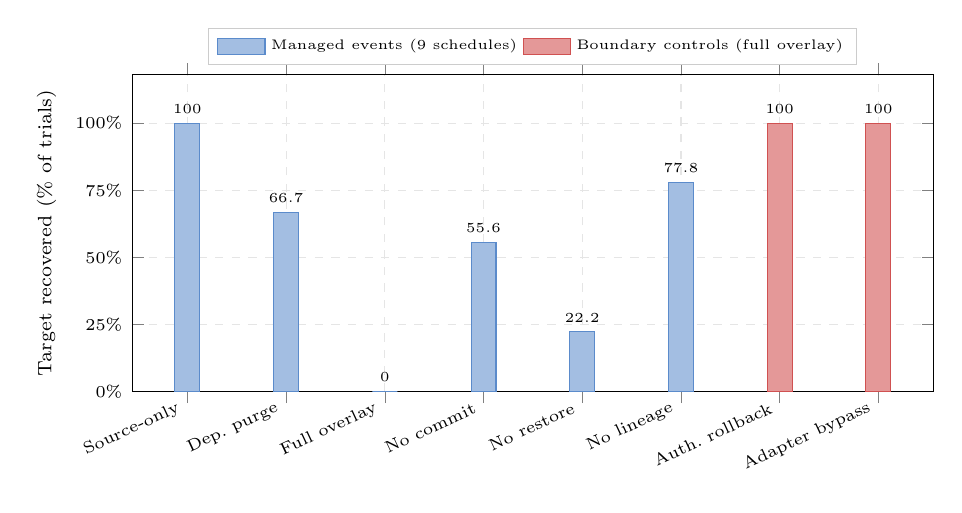
\begin{tikzpicture}
\begin{axis}[
  width=0.97\columnwidth, height=5.6cm, ybar, bar width=9pt,
  symbolic x coords={Source-only,Dep.\ purge,Full overlay,No commit,No restore,No lineage,Auth.\ rollback,Adapter bypass}, xtick={Source-only,Dep.\ purge,Full overlay,No commit,No restore,No lineage,Auth.\ rollback,Adapter bypass},
  x tick label style={font=\fontsize{5.6pt}{7pt}\selectfont, rotate=25, anchor=east},
  ytick={0,25,50,75,100}, yticklabel style={font=\fontsize{6.3pt}{8pt}\selectfont},
  yticklabel={\pgfmathprintnumber{\tick}\%},
  ylabel={Target recovered (\% of trials)}, ylabel style={font=\fontsize{6.8pt}{9pt}\selectfont},
  ymin=0, ymax=118, grid=major, grid style={dashed, gray!20},
  nodes near coords, every node near coord/.append style={font=\fontsize{5.4pt}{6.5pt}\selectfont},
  area legend, legend style={font=\fontsize{5.3pt}{6.8pt}\selectfont, draw=gray!40, at={(0.5,1.03)}, anchor=south}, legend columns=2,
  enlarge x limits=0.08]
\addplot[ybar, bar shift=0pt, fill=cblu!45, draw=cblu!80] coordinates {(Source-only,100.0)(Dep.\ purge,66.7)(Full overlay,0.0)(No commit,55.6)(No restore,22.2)(No lineage,77.8)};
\addlegendentry{Managed events (9 schedules)}
\addplot[ybar, bar shift=0pt, fill=cred!50, draw=cred!85] coordinates {(Auth.\ rollback,100)(Adapter bypass,100)};
\addlegendentry{Boundary controls (full overlay)}
\end{axis}
\end{tikzpicture}
\caption{Pooled recovery per configuration, from \texttt{arm-results.csv} (identical on both backends). Blue bars pool all nine managed schedules (1,260 trials per backend). Red bars are the full overlay under each boundary control (140 trials per backend). Both control bars read 100\%: the overlay's zero is conditional on the current authority being intact and every write path being guarded.}
\Description{Bar chart of the percentage of trials in which the deleted target was recovered. Source-only 100.0; Dep. purge 66.7; Full overlay 0.0; No commit 55.6; No restore 22.2; No lineage 77.8; boundary controls on the full overlay: Auth. rollback 100; Adapter bypass 100.}
\label{fig:bars}
\end{figure}

\subsection{Active files, external fixtures, and utility}
In all 2,520 full-overlay managed trials, the unrelated project record and all background records were preserved, and background retrieval rankings equaled the no-target baseline. Mean gold-session recall at three was 0.8876 across 280 backend--episode observations. This is an absolute retrieval diagnostic, not an LLM answer-accuracy estimate or an independent sample of 280 conversations. Retained fault-replay fixtures contain the target throughout the experiment. The result is therefore a distinction between active-store absence and retained-copy recoverability, rather than a claim that all information is gone.

\subsection{Operation cost}
Median full-overlay deletion took 35.78 ms on SQLite WAL and 22.59 ms on JSON files in this shared-host run. The corresponding one-time-purge medians were 34.11 ms and 20.98 ms. Table~\ref{tab:timing} gives measured medians and 95th percentiles; these timings should not be generalized to remote stores or loaded production agents.
\begin{table}[t]
\caption{Deletion operation timing from the shared-host batch run. Values include this prototype's persistence, cleanup, and index rebuild. They are informational, not isolated system-performance estimates.}
\label{tab:timing}
\centering\small\setlength{\tabcolsep}{3pt}
\begin{tabular}{llrr}
\toprule
Backend & Configuration & \shortstack[r]{Median\\(ms)} & \shortstack[r]{95th pctl.\\(ms)} \\
\midrule
SQLite WAL & Dependency purge & 34.11 & 72.63 \\
SQLite WAL & Full overlay & 35.78 & 78.76 \\
JSON files & Dependency purge & 20.98 & 33.29 \\
JSON files & Full overlay & 22.59 & 37.99 \\
\bottomrule
\end{tabular}
\end{table}

\subsection{Boundary-control failures}
Authority rollback and adapter bypass each restored the target in all 140 episodes on both backends: 560/560 boundary trials. All retained replay fixtures remained recoverable, including during successful active-store deletion. The authority-rollback result rules out a stronger interpretation in which the ordinary memory snapshot somehow proves its own currency. If the current authority is also reset, the prototype cannot distinguish an old authorization from a valid one. Adapter bypass likewise shows that a control plane must cover every publication path.

\section{Discussion}
\subsection{Revocation is a standing condition}
A one-time purge changes the store at deletion time. An epoch guard changes whether subsequent state is admissible. These are complementary obligations: removing derivatives closes current copies, while commit and restore enforcement prevent some future copies. The no-lineage arm demonstrates why preventing later writes cannot repair an already retained derivative by itself.

This interpretation is consistent with the known building blocks in prior work and does not require calling an epoch novel. The practical value of the experiment lies in an explicit contract, cross-adapter tests, and visible failure assumptions. An overlay becomes useful only if actual integrations preserve those assumptions.

\subsection{Deletion receipts and claim language}
A receipt should identify scope, authority generation, managed adapters, operations, unresolved copies, and audit coverage. A successful active scan can justify a statement about the scanned files and methods. It cannot justify a statement about provider logs, model weights, unallocated disk sectors, or retained backups. A signature authenticates a receipt's author; it does not prove that every copy was erased.

Our measured fixture recoverability illustrates a necessary reporting distinction. A restore guard can achieve an active-use contract even when a retained old copy contains the information. A system promising complete recoverability elimination would need an additional policy for registered backups, key management, remote replicas, and underlying media. Those policies are not implemented here.

\subsection{Scope lineage and semantic inference}
Correct scope labels make a deterministic purge tractable. Missing or incorrect labels can cause both leakage and collateral removal. The present artifacts inherit known labels; there is no automatic semantic lineage detector. Real summaries mixing several projects require either whole-artifact removal or selective reconstruction. An adversarially incorrect label can evade this overlay.

Moreover, an unchanged retained record can imply a deleted fact. The exact-target copy test does not measure this inferential channel. A follow-up LLM experiment should use independently authored semantic preferences, never-exposed and length-matched sham worlds, repeated generation, and separate forensic evidence. Its endpoint should be measured rather than inferred from literal preference removal.

\section{Threats to Validity}
\paragraph{Construct validity.} The derivative layers are deterministic records; the checkpoint is not a model-weight checkpoint or KV cache. Retrieval uses a hashed lexical projection and payload inspection. Literal absence does not imply semantic non-influence. The term ``agent memory'' describes the external substrate under study, not a full autonomous agent execution.

\paragraph{Internal validity.} The test coordinator serializes operations and injects specific interleavings. It does not validate a true asynchronous transaction protocol. Shared-host parallel execution and Windows file-sharing behavior affect timings. Both adapters use common overlay logic, so agreement supports adapter consistency rather than independent implementation replication. The source-only positive control is weaker than a complete native scope-delete API; the dependency-purge arm is the meaningful one-time-cleanup baseline.

\paragraph{External validity.} The corpus backgrounds are public conversational-memory examples, but the inserted projects, scope labels, and fault schedules are controlled. The experiment samples a small LoCoMo release and oracle rather than full LongMemEval-S histories. It does not represent all memory vendors, remote services, or user behavior. It estimates performance on a deterministic challenge grid, not natural fault incidence.

\paragraph{Forensic coverage.} Active scans inspect reachable adapter files. They do not guarantee physical-media sanitization, page-cache removal, power-loss recovery, or remote erasure. The numerical-vector cache used to accelerate repeated computation is not subjected to a neural inversion audit. Replay fixtures and result provenance intentionally retain evaluative information.

\paragraph{Statistical validity.} Multiple events reuse each episode, and two LoCoMo questions share a conversation. Finite-grid counts and descriptive bootstrap contrasts should not be promoted to population-level significance. This study does not conduct a behavioral equivalence or generated-answer noninferiority test.

\paragraph{Novelty and publication status.} Several closely related 2026 works are preprints or incompletely accessible. Broader independent searches and full-method review remain necessary before claiming priority. The manuscript is a research draft based on the reported experiment, not an accepted ACM publication or a certified deletion system.

\section{Data, Artifacts, and Research Integrity}
The source downloads retain revision-pinned URLs, SHA-256 values, sizes, and upstream license/card files. LongMemEval's downloaded release declares MIT; LoCoMo declares CC BY-NC 4.0. The experiment package preserves those distinctions. No real private credential is used and no attempt is made to identify individuals. No user conversations are sent to an inference provider during this study.

The downloadable artifact contains the protocol, Python reference implementation, tests, raw trial JSONL, per-event and per-arm CSV summaries, analysis code, and validation reports. Corpus files remain in the companion data directory, and the small Overleaf package excludes their large payloads. Reproduction instructions fetch the recorded public revisions and verify hashes. A publication release should also provide a persistent repository or archival identifier; none is invented here.

AI assistance was used to develop code, analysis, and manuscript text. All numerical claims are generated from recorded executable outcomes and checked against the result files. Human authors must independently review attribution, experimental adequacy, and venue-specific requirements before submission. No author affiliation, funding award, ethics approval, DOI, acceptance, or review result is fabricated.

\section{Conclusion}
The controlled experiment distinguishes removing currently materialized copies from maintaining revocation during later operations. The full overlay prevented active recovery in 2,520 managed trials across two backends, while one-time dependency purge failed under six of nine lifecycle schedules. The failures under authority rollback and adapter bypass expose the assumptions behind those results. Retained replay copies remain recoverable, so the appropriate claim is bounded active-memory revocation. The next research step is to reproduce the protocol in real agent-memory frameworks and extend measurement to LLM behavior and semantic inference; the present storage outcomes cannot substitute for those measurements.

\begin{thebibliography}{12}
\bibitem{chen2026} Lei (Rachel) Chen et al. 2026. Deployment-Time Memorization in Foundation-Model Agents. ICML MemFM workshop listing; arXiv:2606.10062v2. \url{https://arxiv.org/abs/2606.10062}.
\bibitem{yang2026} Dongxu Yang. 2026. Control-Plane Placement Shapes Forgetting: An Architectural Study of Agent Memory Across Thirteen System Configurations. arXiv:2606.15903v2. \url{https://arxiv.org/abs/2606.15903}.
\bibitem{liu2026} Jiabei Liu and Mingyang Li. 2026. Deletion Is Not Forgetting: Behavioral Residuals of Deleted Memories in Stateful LLM Agents. SSRN working paper, posted September 7. Abstract consulted. \url{https://papers.ssrn.com/sol3/papers.cfm?abstract_id=7428966}.
\bibitem{memleak2026} Kuan Wang and Chao Zhang. 2026. MemLeak: Diagnosing Information Leaks in Multimodal Agent Memory. arXiv:2606.29788v1. \url{https://arxiv.org/abs/2606.29788}.
\bibitem{dsit2026} Department for Science, Innovation and Technology. 2026. Thematic Review and Gap Analysis on AI Security. Lancaster University commissioned review, July 10. \url{https://www.gov.uk/government/publications/thematic-review-and-gap-analysis-on-ai-security}.
\bibitem{chourasia2023} Rishav Chourasia and Neil Shah. 2023. Forget Unlearning: Towards True Data-Deletion in Machine Learning. In \emph{Proceedings of ICML}, PMLR 202, 6028--6073. \url{https://proceedings.mlr.press/v202/chourasia23a.html}.
\bibitem{ding2026} Zihao Ding, Jun Huang, and Liang Dong. 2026. When Unlearning Fails: Reliable Data Deletion under Post-Training in Agent Networks. arXiv:2607.28829v1. \url{https://arxiv.org/abs/2607.28829}.
\bibitem{shen2026} Chen Shen. 2026. What Eviction Destroys: A Restore-Counterfactual Audit of Forgetting in Agent Memory. arXiv:2609.08279v1. \url{https://arxiv.org/abs/2609.08279}.
\bibitem{longmemeval} Di Wu, Hongwei Wang, Wenhao Yu, Yuwei Zhang, Kai-Wei Chang, and Dong Yu. 2024. LongMemEval: Benchmarking Chat Assistants on Long-Term Interactive Memory. arXiv:2410.10813; accepted at ICLR 2025 according to the official repository. \url{https://github.com/xiaowu0162/LongMemEval}.
\bibitem{locomo} Snap Research. 2024. LoCoMo: Official Dataset and Code Repository. Dataset release used: \texttt{data/locomo10.json}; attribution retained in the companion artifact. \url{https://github.com/snap-research/locomo}.
\bibitem{sqlitepragma} SQLite Project. n.d. PRAGMA Statements: secure\_delete and wal\_checkpoint. Official documentation, accessed October 4, 2026. \url{https://www.sqlite.org/pragma.html}.
\bibitem{sqlitewal} SQLite Project. n.d. Write-Ahead Logging. Official documentation, accessed October 4, 2026. \url{https://www.sqlite.org/wal.html}.
\end{thebibliography}

\appendix
\section{Executable Protocol and Reproduction}
Use Python 3.12 with NumPy for analysis. From the companion outputs directory, run the unit tests, then the experiment, then analysis. The frozen reference results were produced in four shards; the provided runner supports a single-process reproduction and the artifact instructions describe merging its output. Exact non-timing outcomes should agree; timings are hardware and host-load dependent.

\begin{Verbatim}[fontsize=\footnotesize,breaklines=true,breakanywhere=true]
python -m unittest discover -s experiment -p test_overlay.py -v
python experiment/run_experiment.py --out experiment/reproduction
python experiment/analyze.py --results experiment/reproduction
\end{Verbatim}
The reference protocol SHA-256 begins \texttt{a978d6b90b5cf899}. Full SHA-256 values, source hashes, input hashes, and environment metadata are retained in the JSON manifests. Write fresh results to a separate directory rather than overwrite the reference observations.

\section{Interpreting the Recorded Outcomes}
\begin{table}[h]
\caption{Result fields and their boundaries.}
\begin{tabular}{>{\raggedright\arraybackslash}p{0.34\linewidth}>{\raggedright\arraybackslash}p{0.57\linewidth}}
\toprule
Recorded quantity & What it establishes \\
\midrule
Record recovery & Exact target in active record/index payload. \\
Persisted-byte recovery & Exact target in currently reachable adapter files. \\
Retrieval at three & Exact target in the top-three hashed-lexical payloads. \\
Preference residue & Literal project-preference sentence remains; no LLM effect measured. \\
Unchanged background & Retained records are structurally equal to their initial content. \\
Gold-session recall & Fraction of evaluator-labeled evidence sessions in top-three raw results. \\
Fixture recovery & Pre-deletion replay copy still contains the target; erasure is incomplete outside active scope. \\
\bottomrule
\end{tabular}
\end{table}
\end{document}
